\section{Results}
(Distribuzione dati fatta tenendo conto della geometria (3D) del
problema e giustificandola rispetto al vantaggio che fornisce in
termini di rapporto calcolo/comunicazione.) 

We illustrate the behaviour of the AMG preconditioner and the INVK
solver on GPUs  by showing the results obtained on a linear system
arisen from a groundwater modelling application developed at the
Juelich Supercomputing Centre (JSC)  dealing with numerical simulation
of the filtration of 3D incompressible single-phase flows through
anisotropic porous media. It is an elliptic equation with no flow
boundary conditions. The linear systems arises from the discretization
of the equation performed by a cell-centered finite colume scheme
(two-point flux approximation) on a Cartesian grid, with nonzero
entries distributed over seven diagonals. In these tests, we will
consider a homogeneous permeability tensor.  
Weak scalability tests are performed, using approximately 2 millions
equations per process. The total dimension ranges from 2 millions up
to 256 millions of equations~\ref{np-dim}. 
This application comes from the framework of the Horizon 2020 EoCoE
Project 

We ran experiments on the JURECA supercomputer at the Juelich
Supercomputing Centre (JSC).  Each GPU compute node consists of two
NVIDIA Tesla K80 GPUs with a dual-GPU design, for a total of four
available GPU devices per compute nodes.  
We used PSBLAS 3.5 (combined with its extension plugin for extended
matrix formats and GPU plugin) and MLD2P4 2.1 (combined with AINV
plugin),  compiled with  GNU compilers (C and Fortran) version 5.4.0,
MVAPICH2 version 2.3 and with CUDA 8.0.61. 

Linear systems are solved using Conjugated Gradient (CG) and the
stopping criterion is based on the ratio bewteen 2-norms of the
residual and the right-hand side vector (when smaller than
$10^{-6}$). CG is use in conjuction with a V-cycle preconditioner. We
consider two different configurations. In the first case the V-cycle
preconditioner applies 1 pre and post sweep of Block Jacobi smoother
with INVK (approximate inverse based on the inversion of triangular
factors based on a positional drop strategy) as a solver. In the
second configuration it applies 2 per and post sweeps of Jacobi
solver. In both cases, we use 10 sweeps of Block Jacobi with INVK  as
coarsest level solver.   
For each configuration, we ran tests only on CPUs (with matrices in
CSR format) and using CPUs+GPUs (with matrices in ELG format). This
allows us to quantify the gain in efficiency in using GPUs.   

First, we show results for the case using BJAC(INVK) smoother on the
inner levels. In table \ref{gpu-invk} the last column shows the
speed-up of the solver phase on the gpu with respect to the cpu solve
time.   


\begin{table}[h!]
\centering
\caption{Numerical results for CG + ML preconditioner, runs on CPUs, with 1 sweep of BJAC(INVK) as smoother on inner levels.}
\label{cpu-invk}

\begin{tabular}{rrrrrrr}
\multicolumn{1}{l}{np} & \multicolumn{1}{l}{levels} & \multicolumn{1}{l}{It} & \multicolumn{1}{l}{\begin{tabular}[c]{@{}l@{}}Prec    \\   time (s)\end{tabular}} & \multicolumn{1}{l}{\begin{tabular}[c]{@{}l@{}}Solve  \\  Time (s)\end{tabular}} & \multicolumn{1}{l}{\begin{tabular}[c]{@{}l@{}}Time per \\ Iteration (s)\end{tabular}} & \multicolumn{1}{l}{\begin{tabular}[c]{@{}l@{}}Total  \\   Time (s)\end{tabular}} \\ \hline
1     & 4    & 14  & 17.74  & 4.42   & 0.32   & 22.15   \\
2     & 4    & 15  & 19.43  & 5.05   & 0.34   & 24.47   \\
4     & 4    & 18  & 21.85  & 6.96   & 0.39   & 28.81  \\
8     & 4    & 20  & 28.32  & 8.05   & 0.40   & 36.37  \\
16    & 4    & 24  & 26.38  & 9.59   & 0.40   & 35.98  \\
32    & 4    & 29  & 23.52  & 11.42  & 0.39   & 34.93  \\
64    & 4    & 34  & 29.61  & 14.21  & 0.42   & 43.82  \\
128   & 5    & 29  & 28.39  & 13.19  & 0.45   & 41.58 \\
\end{tabular}
\end{table}

\begin{table}[h!]
\centering
\caption{Numerical results for CG + ML preconditioner, runs on GPUs, with 1 sweep of BJAC(INVK) as smoother on inner levels.}
\label{gpu-invk}

\begin{tabular}{rrrrrrrr}
\multicolumn{1}{l}{np} & \multicolumn{1}{l}{levels} & \multicolumn{1}{l}{It} & \multicolumn{1}{l}{\begin{tabular}[c]{@{}l@{}}Prec    \\   time (s)\end{tabular}} & \multicolumn{1}{l}{\begin{tabular}[c]{@{}l@{}}Solve  \\  Time (s)\end{tabular}} & \multicolumn{1}{l}{\begin{tabular}[c]{@{}l@{}}Time per \\ Iteration (s)\end{tabular}} & \multicolumn{1}{l}{\begin{tabular}[c]{@{}l@{}}Total  \\   Time (s)\end{tabular}} & \multicolumn{1}{l}{\begin{tabular}[c]{@{}l@{}}Speed up\\ cpu/gpu\end{tabular}} \\ \hline
1   & 4  & 14 & 18.80  & 0.45 & 0.03  & 19.24  & 9.92  \\
2   & 4  & 15 & 20.55  & 0.54 & 0.04  & 21.09  & 9.40   \\
4   & 4  & 18 & 22.84  & 0.69 & 0.04  & 23.54  & 10.08  \\
8   & 4  & 20 & 29.18  & 0.86 & 0.04  & 30.03  & 9.40   \\
16  & 4  & 24 & 27.38  & 1.12 & 0.05  & 28.50  & 8.57   \\
32  & 4  & 29 & 23.74  & 1.29 & 0.04  & 25.02  & 8.85   \\
64  & 4  & 34 & 30.53  & 1.79 & 0.05  & 32.32  & 7.94   \\
128 & 5  & 29 & 29.48  & 2.22 & 0.08  & 31.70  & 5.94  \\                                                                        
\end{tabular}
\end{table}




Secondly, the results for the case using two sweep of a Jacobi smoother on inner levels.

\begin{table}[h!]
\centering
\caption{Numerical results for CG + ML preconditioner, runs on CPUs, with 2 sweeps of JACOBI as smoother on inner levels.}
\label{cpu-jac}

\begin{tabular}{rrrrrrr}
\multicolumn{1}{l}{np} & \multicolumn{1}{l}{levels} & \multicolumn{1}{l}{It} & \multicolumn{1}{l}{\begin{tabular}[c]{@{}l@{}}Prec    \\   time (s)\end{tabular}} & \multicolumn{1}{l}{\begin{tabular}[c]{@{}l@{}}Solve  \\  Time (s)\end{tabular}} & \multicolumn{1}{l}{\begin{tabular}[c]{@{}l@{}}Time per \\ Iteration (s)\end{tabular}} & \multicolumn{1}{l}{\begin{tabular}[c]{@{}l@{}}Total  \\   Time (s)\end{tabular}} \\ \hline
1   & 4 & 19  & 2.83 & 3.76  & 0.20  & 6.59  \\
2   & 4 & 21  & 3.65 & 4.57  & 0.22  & 8.23  \\
4   & 4 & 20  & 4.21 & 5.13  & 0.26  & 9.35  \\
8   & 4 & 25  & 4.75 & 6.58  & 0.26  & 11.33 \\
16  & 4 & 27  & 4.97 & 7.21  & 0.27  & 12.18 \\
32  & 4 & 31  & 4.88 & 8.21  & 0.26  & 13.09 \\
64  & 4 & 37  & 5.79 & 10.20 & 0.28  & 16.00 \\
128 & 5 & 31  & 6.72 & 11.16 & 0.36  & 17.88 \\                                                                          
\end{tabular}
\end{table}


\begin{table}[]
\centering
\caption{Numerical results for CG + ML preconditioner, runs on GPUs, with 2 sweeps of JACOBI as smoother on inner levels.}
\label{gpu-jac}
\begin{tabular}{rrrrrrrr}
\multicolumn{1}{l}{np} & \multicolumn{1}{l}{levels} & \multicolumn{1}{l}{It} & \multicolumn{1}{l}{\begin{tabular}[c]{@{}l@{}}Prec    \\   time (s)\end{tabular}} & \multicolumn{1}{l}{\begin{tabular}[c]{@{}l@{}}Solve  \\  Time (s)\end{tabular}} & \multicolumn{1}{l}{\begin{tabular}[c]{@{}l@{}}Time per \\ Iteration (s)\end{tabular}} & \multicolumn{1}{l}{\begin{tabular}[c]{@{}l@{}}Total  \\   Time (s)\end{tabular}} & \multicolumn{1}{l}{\begin{tabular}[c]{@{}l@{}}Speed up\\ cpu/gpu\end{tabular}} \\ \hline
1   & 4  & 19  & 3.13  & 0.40  & 0.02  & 3.53  & 9.39  \\
2   & 4  & 21  & 4.06  & 0.52  & 0.02  & 4.59  & 8.73  \\
4   & 4  & 20  & 4.65  & 0.63  & 0.03  & 5.28  & 8.16  \\
8   & 4  & 25  & 5.20  & 0.85  & 0.03  & 6.05  & 7.74  \\
16  & 4  & 27  & 5.39  & 1.02  & 0.04  & 6.42  & 7.06  \\
32  & 4  & 31  & 5.35  & 1.24  & 0.04  & 6.59  & 6.61  \\
64  & 4  & 37  & 6.25  & 1.71  & 0.05  & 7.96  & 5.98  \\
128 & 5  & 31  & 7.19  & 2.23  & 0.07  & 9.43  & 5.00  \\
\end{tabular}
\end{table}


\begin{figure}
\begin{center}
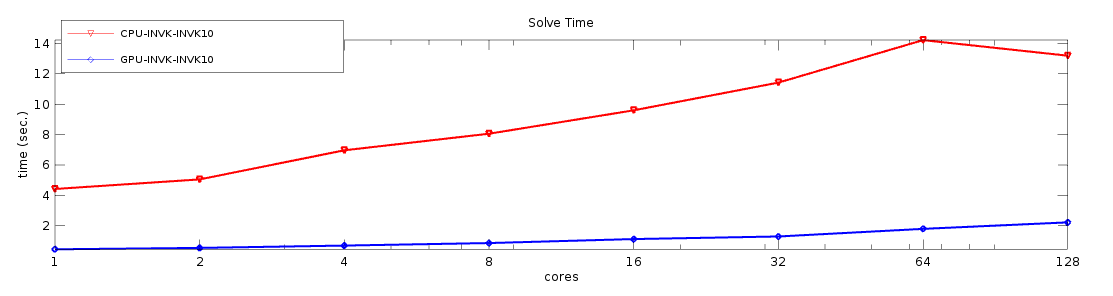
\includegraphics[width=.9\textwidth]{graf_invk.png}
\end{center}
\caption{INVK-INVK}
\end{figure}

\begin{figure}
\begin{center}
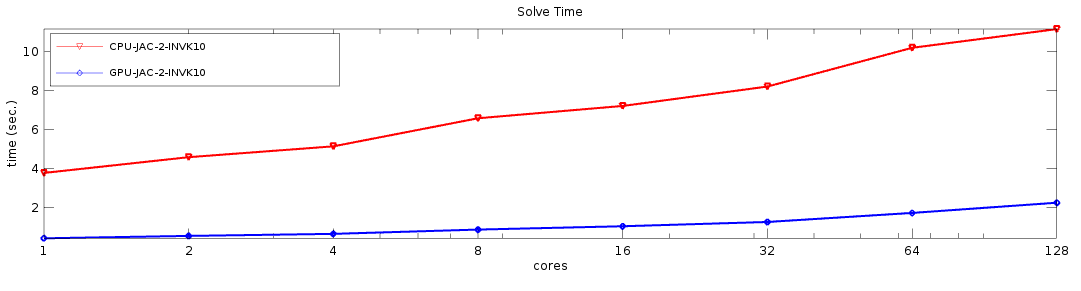
\includegraphics[width=.9\textwidth]{graf_jac2.png}
\end{center}
\caption{JAC2-INVK}
\end{figure}
